\chapter{Quadrilateral Quality Metrics}

All the metrics in this section are defined on a quadrilateral element with vertices
shown in Figure~\ref{f:quad}. Furthermore, we define the following edge vectors for
convenience. Note that each edge has two versions, one defined by its endpoints and
another indexed by sequential integers:
\begin{equation*}
\begin{array}{lcl}
\vec L_0 &=& \vec P_1 - \vec P_0\\
\vec L_1 &=& \vec P_2 - \vec P_1\\
\vec L_2 &=& \vec P_3 - \vec P_2\\
\vec L_3 &=& \vec P_0 - \vec P_3
\end{array}\rule{10em}{0pt}
\begin{array}{lcl}
\vec L_{01} &=& \vec P_1 - \vec P_0\\
\vec L_{12} &=& \vec P_2 - \vec P_1\\
\vec L_{23} &=& \vec P_3 - \vec P_2\\
\vec L_{30} &=& \vec P_0 - \vec P_3.
\end{array}
\end{equation*}

The quadrangle edge lengths are denoted as follows:
\[
L_0 = \normvec{L_0}\quad
L_1 = \normvec{L_1}\quad
L_2 = \normvec{L_2}\quad
L_3 = \normvec{L_3}
\]
and the largest and smallest edge lengths are, respectively,
\[
L_{\min} = \min\left(L_0, L_1, L_2, L_3\right)
  \rule{2em}{0pt}
L_{\max} = \max\left(L_0, L_1, L_2, L_3\right)
\]

The diagonals of a quadrilateral are denoted
\begin{equation*}
\begin{array}{lcl}
\vec D_0 &=& \vec P_2 - \vec P_0
\end{array}\rule{10em}{0pt}
\begin{array}{lcl}
\vec D_1 &=& \vec P_3 - \vec P_1
\end{array}
\end{equation*}
and the longest diagonal has length
\[
D_{\max} = \max\left\{ \normvec{D_0}, \normvec{D_1} \right\}.
\]

\begin{figure}[htb]
  \centering
  \subfigure[Vertices of a quadrilateral.]{\includegraphics[width=2in]{quad}}
  \subfigure[Principal axis vectors.]{\includegraphics[width=2in]{quad-axes}}
  \caption{A quadrilateral showing notation used in metric definitions.%
                                                                  \label{f:quad}}
\end{figure}

The principal axes are
\begin{equation*}
\begin{array}{lcl}
\vec X_1 &=& \left(\vec P_1 - \vec P_0\right) + \left(\vec P_2 - \vec P_3\right)\\
\vec X_2 &=& \left(\vec P_2 - \vec P_1\right) + \left(\vec P_3 - \vec P_0\right)
\end{array}
\end{equation*}
and the cross derivatives of the map from parametric to world space are oriented along
\begin{equation*}
\begin{array}{lcl}
\vec X_{12} &=& \left(\vec P_0 - \vec P_1\right) + \left(\vec P_2 - \vec P_3\right) =\\
\vec X_{21} &=& \left(\vec P_0 - \vec P_3\right) + \left(\vec P_2 - \vec P_1\right).
\end{array}
\end{equation*}

Each corner has a normal vector associated with it
\begin{equation*}
\begin{array}{lcl}
\vec N_0 &=& \vec L_3 \times \vec L_0\\
\vec N_1 &=& \vec L_0 \times \vec L_1
\end{array}
\rule{10em}{0pt}
\begin{array}{lcl}
\vec N_2 &=& \vec L_1 \times \vec L_2\\
\vec N_3 &=& \vec L_2 \times \vec L_3
\end{array}
\end{equation*}
and these vectors can be normalized to unit length:
\begin{equation*}
\begin{array}{lcl}
\hat n_0 &=& \dfrac{\vec N_0}{\normvec{ N_0}}\\
\hat n_1 &=& \dfrac{\vec N_1}{\normvec{ N_1}}
\end{array}
\rule{10em}{0pt}
\begin{array}{lcl}
\hat n_2 = \dfrac{\vec N_2}{\normvec{ N_2}}\\
\hat n_3 = \dfrac{\vec N_3}{\normvec{ N_3}}.
\end{array}
\end{equation*}

In addition to corner normals, we can define a ``center'' normal
\begin{equation*}
\vec N_{c} = \vec X_1 \times \vec X_2
\end{equation*}
and its unit-length companion
\begin{equation*}
\hat n_{c} = \frac{\vec N_{c}}{\normvec{ N_{c}}}
\end{equation*}
In the event that the vertices of the quadrilateral are all
contained in the same plane, all the unit normals will be
equivalent (i.e., $\hat n_0 = \hat n_1 = \hat n_2 = \hat n_3 = \hat n_c$).

\begin{figure}[htb]
  \centering
  \includegraphics[width=2in]{quad-vertex-areas}
  \caption{Areas associated with each quadrilateral vertex.%
                                                    \label{f:quad-vertex-areas}}
\end{figure}

It is often useful to partition the quadrilateral into four areas, one
associated with each vertex. These areas are denoted
\begin{equation*}
\alpha_k = \hat n_c \cdot \vec N_k\rule{10em}{0pt}\forall k\in\{0,1,2,3\}
\end{equation*}
and are shown in Figure~\ref{f:quad-vertex-areas}.
If $\vec N_c = \vec 0$, then the signed corner areas are undefined,
and all the metrics which depend on $\alpha_k$ are undefined.
In this case, we set $\alpha_k = 0$ for $k=0,1,2,3$.
When $\alpha_k \leq 0$ for any one or more $k$, the quadrilateral
is degenerate.
This occurs when
an element is so small its edge length approach the machine epsilon or
when its vertices are collinear or
when its vertices define a concave quadrilateral.

% -------------------Metric Table-------------------
\newcommand{\quadmetrictable}[8]{%
  \begin{center}
  \begin{tabular}{ll}
    \multicolumn{2}{r}{\textbf{\sffamily\Large quadrilateral #1}}\\\hline
    Dimension:             & #2\\ 
    Acceptable Range:      & #3\\ 
    Normal Range:          & #4\\ 
    Full Range:            & #5\\ 
    $q$ for unit square:   & #6\\
    Reference:             & #7\\
    \verd\ function:       & \texttt{#8}\\ \hline
  \end{tabular} 
  \end{center}
}

\newpage %---------------------------Area-----------------------------
\section{Area\label{s:quad-area}}

Signed area, defined as
\[
q = \frac {1} {4} \sum_{i=0}^3 \alpha_i
\]
is useful for two purposes: first, the sign can indicate elements
that have vertices ordered incorrectly or arranged in a concave
pattern; and second, the magnitude can be used to identify
elements that are too small for accurate analysis.
Figure~\ref{f:quad-areas} shows how each vertex area contributes to
the total area of a quadrilateral.

\begin{figure}[htb]
  \centering
  \includegraphics[width=2in]{quad-areas}
  \caption{The areas associated with each vertex may be summed and
           weighted to get the area of the entire quadrilateral.%
                                                                  \label{f:quad-areas}}
\end{figure}

\quadmetrictable{area}%
{$L^2$}%                                    Dimension
{$[0,DBL\_MAX]$}%                           Acceptable range
{$[0,DBL\_MAX]$}%                           Normal range
{$[-DBL\_MAX,DBL\_MAX]$}%                   Full range
{$1$}%                                      Unit square
{--}%                                       Citation
{v\_quad\_area}%                            Verdict function name


\newpage %---------------------------Aspect Ratio-----------------------------
\section{Aspect Ratio\label{s:quad-aspect-ratio}}

The aspect ratio of a quadrilateral is: 
\[
q = \frac{L_{\max}(L_0+L_1+L_2+L_3)}{4A},
\]
where $A$ is the area of the quadrilateral. 

Note that, strictly speaking, the aspect ratio is usually defined for
simplicial elements as the ratio of the maximum edge length to the
inradius (\emph{cf.}~\S\ref{s:tri-aspect-ratio} and
~\S\ref{s:tet-aspect-ratio}). However, a planar quadrilateral does not
have, in general, an inscribed circle: such an incircle exists if and
only if $L_0+L_2=L_1+L_3$. Nonetheless, using the expression
of the triangle aspect ratio as given
in~\eqref{eq:triangle_aspect_ratio}, that is, with no explicit
reference to the inradius but only to the perimeter and the area, one
can then directly extrapolate to obtain a meaningful definition of the
quadrangle aspect ratio.

\trimetrictable{aspect ratio}%
{$1$}%                                                Dimension
{$[1,1.3]$}%                                          Acceptable range
{$[1,DBL\_MAX]$}%                                     Normal range
{$[1,DBL\_MAX]$}%                                     Full range
{$1$}%                                                Unit square
{\cite{pebay:04}}%                                    Reference(s)                   
{v\_quad\_aspect\_ratio}%                             Verdict function name


\newpage %---------------------------Condition-----------------------------
\section{Condition}

\[
q = \frac{1}{2} \max \left\{  \frac {\normvec{L_0}^2 + \normvec{L_3}^2 } { \alpha_0 },
                        \frac {\normvec{L_1}^2 + \normvec{L_0}^2 } { \alpha_1 },
                        \frac {\normvec{L_2}^2 + \normvec{L_1}^2 } { \alpha_2 },
                        \frac {\normvec{L_3}^2 + \normvec{L_2}^2 } { \alpha_3 } 
                \right\}
\]

Note that if $\alpha_i< DBL\_MIN$, we set $q = DBL\_MAX$.

\quadmetrictable{condition}%
{$1$}%                                      Dimension
{$[1,4]$}%                                  Acceptable range
{$[1,DBL\_MAX]$}%                           Normal range
{$[1,DBL\_MAX]$}%                           Full range
{$1$}%                                      Unit square
{\cite{knu:00}}%                            Citation
{v\_quad\_condition}%                       Verdict function name


\newpage %---------------------------Distortion-----------------------------
\section{Distortion}

Let $A$ be the area as defined in \S\ref{s:quad-area}
and $A_m = 4$ be the area of a ``master'' quadrilateral with vertices
\[
\begin{array}{lcrcrcrl}
  \vec P_0 &= (&-1&,&-1&,& 0&)\\
  \vec P_1 &= (& 1&,&-1&,& 0&)\\
  \vec P_2 &= (& 1&,& 1&,& 0&)\\
  \vec P_3 &= (&-1&,& 1&,& 0&).
\end{array}
\]
Now define $|J|$ as the minimum value of the
determinant of the Jacobian evaluated at all Gauss points of the element.
The distortion is then
\[
q = \frac{|J| A_m}{A} = \frac{4|J|}{A}.
\]
Distortion is a measure of how well-behaved the mapping from
parameter space to world coordinates is.

\quadmetrictable{distortion}%
{$1$}%                                      Dimension
{$[0.5,1]$}%                                Acceptable range
{$[0,1]$}%                                  Normal range
{$[-DBL\_MAX,DBL\_MAX]$}%                   Full range
{$1$}%                                      Unit square
{\cite{ideas:xx}}%                          Citation
{v\_quad\_distortion}%                      Verdict function name


\newpage %---------------------------Edge Ratio-----------------------------
\section{Edge Ratio}

The edge ratio of a quadrilateral is the ratio of its longest and shortest edge lengths:
\[
  q = \frac{L_{\max}}{L_{\min}}.
\]

\quadmetrictable{edge ratio}%
{$1$}%                                      Dimension
{$[1,1.3]$}%                                Acceptable range
{$[1,DBL\_MAX]$}%                           Normal range
{$[1,DBL\_MAX]$}%                           Full range
{$1$}%                                      Square
{\cite{pebay:04}}%                          Citation
{v\_quad\_edge\_ratio}%                     Verdict function name


\newpage %---------------------------Jacobian-----------------------------
\section{Jacobian}

The minimum Jacobian computed at each vertex is used:
\[
q = \min_{i\in\{0,1,2,3\}} \left\{ \alpha_i \right\}
\]

\quadmetrictable{Jacobian}%
{$L^2$}%                                    Dimension
{$[0.DBL\_MAX]$}%                           Acceptable range
{$[0,DBL\_MAX]$}%                           Normal range
{$[-DBL\_MAX,DBL\_MAX]$}%                   Full range
{$1$}%                                      Unit square
{\cite{knu:00}}%                            Citation
{v\_quad\_jacobian}%                        Verdict function name


\newpage %---------------------------Maximum Aspect Frobenius-----------------------------
\section{Maximum Aspect Frobenius}

For quadrilaterals, there is not a unique definition of the aspect Frobenius.
Instead, we use the aspect Frobenius
defined for triangles (see section~\S\ref{s:tri-aspect-Frobenius}).
Consider the four triangles formed by pairs of neighboring quadrilateral edges.
Given three counterclockwise, consecutively ordered quadrilateral vertices $i$, $j$, and $k$
denote the triangular aspect frobenius $F_{ijk}$.
To obtain a single value for the metric, we take the maximum of the four unique triangular aspects
\[
  q = \max\left(F_{301}, F_{012}, F_{123}, F_{230}\right).
\]

\quadmetrictable{maximum aspect frobenius}%
{$1$}%                                      Dimension
{$[1,1.3]$}%                                Acceptable range
{$[1,DBL\_MAX]$}%                           Normal range
{$[1,DBL\_MAX]$}%                           Full range
{$1$}%                                      Unit square
{\cite{pebay:04}}%                          Citation
{v\_quad\_max\_aspect\_frobenius}%          Verdict function name


\newpage %---------------------------Maximum Angle-----------------------------
\section{Maximum Angle}

In order to properly compute the included angle, we'll need to
correct for incorrectly oriented elements.
Let
\[
s_i = \left\{ \begin{array}{ll}
  1\rule{2em}{0pt} & \alpha_i < 0\\
  0                & \alpha_i \geq 0
  \end{array}\right.
\]
The included angle between two neighboring edges is
\[
\theta_i = (-1)^{s_i} \arccos{ \left( - \frac {\vec L_{i} \cdot \vec L_{i+1} }
                                {\normvec{L_{i}} \normvec{L_{i+1}}} \right) } 
                                  \left( \frac {180} {\pi} \right) 
           + 360\dgr s_i
\]
where $i\in\{0,1,2,3\}$ and $\vec L_4 = \vec L_0$.
We take the maximum of this quantity as the value of the metric:
\[
q = \max_{i\in\{0,1,2,3\}}\left\{ \theta_i \right\}
\]

Note that if $\normvec{L_i} \leq DBL\_MIN$ or $\normvec{L_{i+1}} \leq DBL\_MIN$,
\verd\ returns $q = 0\dgr$.

\quadmetrictable{maximum included angle}%
{$A^1$}%                                    Dimension
{$[90\dgr,135\dgr]$}%                       Acceptable range
{$[90\dgr,360\dgr]$}%                       Normal range
{$[0\dgr,360\dgr]$}%                        Full range
{$90\dgr$}%                                 Unit square
{--}%                                       Citation
{v\_quad\_maximum\_angle}%                  Verdict function name


\newpage %---------------------------Maximum Edge Ratio-----------------------------
\section{Maximum Edge Ratio}

\[
q = \max \left\{  \normvec{ X_1 } / \normvec{ X_2 }, 
                  \normvec{ X_2 } / \normvec{ X_1 } \right\} 
\]

Note that if $\normvec{X_1}$ or $\normvec{X_2} < DBL\_MIN$, we set $q = DBL\_MAX$.

\quadmetrictable{maximum edge ratio}%
{$1$}%                                      Dimension
{$[1,1.3]$}%                                Acceptable range
{$[1,DBL\_MAX]$}%                           Normal range
{$[1,DBL\_MAX]$}%                           Full range
{$1$}%                                      Unit square
{\cite{rob:87}}%                            Citation
{v\_quad\_max\_edge\_ratio}%                Verdict function name


\newpage %---------------------------Mean Aspect Frobenius-----------------------------
\section{Mean Aspect Frobenius}

For quadrilaterals, there is not a unique definition of the aspect Frobenius.
Instead, we use the aspect Frobenius
defined for triangles (see section~\S\ref{s:tri-aspect-Frobenius}).
Consider the four triangles formed by pairs of neighboring quadrilateral edges.
Given three counterclockwise, consecutively ordered quadrilateral vertices $i$, $j$, and $k$
denote the triangular aspect frobenius $F_{ijk}$.
To obtain a single value for the metric, we average the four unique triangular aspects
\[
  q = \frac{1}{4}\left(F_{301} + F_{012} + F_{123} + F_{230}\right).
\]

\quadmetrictable{mean aspect frobenius}%
{$1$}%                                      Dimension
{$[1,1.3]$}%                                Acceptable range
{$[1,DBL\_MAX]$}%                           Normal range
{$[1,DBL\_MAX]$}%                           Full range
{$1$}%                                      Unit square
{\cite{pebay:04}}%                          Citation
{v\_quad\_med\_aspect\_frobenius}%          Verdict function name


\newpage %---------------------------Minimum Angle-----------------------------
\section{Minimum Angle}

In order to properly compute the included angle, we'll need to
correct for incorrectly oriented elements.
Let
\[
s_i = \left\{ \begin{array}{ll}
  1\rule{2em}{0pt} & \alpha_i < 0\\
  0                & \alpha_i \geq 0
  \end{array}\right.
\]
The included angle between two neighboring edges is
\[
\theta_i = (-1)^{s_i} \arccos{ \left( - \frac {\vec L_{i} \cdot \vec L_{i+1} }
                                {\normvec{L_{i}} \normvec{L_{i+1}}} \right) } 
                                  \left( \frac {180} {\pi} \right) 
           + 360\dgr s_i
\]
where $i\in\{0,1,2,3\}$ and $\vec L_4 = \vec L_0$.
We take the minimum of this quantity as the value of the metric:
\[
q = \min_{i\in\{0,1,2,3\}}\left\{ \theta_i \right\}
\]

Note that if $\normvec{L_i} \leq DBL\_MIN$ or $\normvec{L_{i+1}} \leq DBL\_MIN$,
\verd\ returns $q = 360\dgr$.

\quadmetrictable{minimum included angle}%
{$A^1$}%                                    Dimension
{$[45\dgr,90\dgr]$}%                        Acceptable range
{$[0\dgr,90\dgr]$}%                         Normal range
{$[0\dgr,360\dgr]$}%                        Full range
{$90\dgr$}%                                 Unit square
{--}%                                       Citation
{v\_quad\_minimum\_angle}%                  Verdict function name


\newpage %---------------------------Oddy-----------------------------
\section{Oddy}

Let $\vec L_4 = \vec L_0$. The Oddy metric is then defined as
\[
q = \max_{i\in\{0,1,2,3\}}\left\{
    \frac{(\normvec{L_i}^2 - \normvec{L_{i+1}}^2)^2 
    + 4 (\vec L_i \cdot \vec L_{i+1})^2}
    {2 \normvec{N_{i+1}}^2 }
  \right\}.
\]
This metric measures the maximum deviation of the metric tensor at the corners of the quadrilateral.

Note that if $\normvec{N_{i+1}}^2 < DBL\_MIN$, we set $q = DBL\_MAX$.

\quadmetrictable{Oddy}%
{$1$}%                                      Dimension
{$[0,0.5]$}%                                Acceptable range
{$[0,DBL\_MAX]$}%                           Normal range
{$[0,DBL\_MAX]$}%                           Full range
{$0$}%                                      Unit square
{\cite{odd:88}}%                            Citation
{v\_quad\_oddy}%                            Verdict function name


\newpage %---------------------------Radius Ratio-----------------------------
\section{Radius Ratio}

Let $h_{\max}$ be the maximum length of all edges and diagonals
\[
  h_{\max} = \max\left(L_{\max},D_{\max}\right)
\]
and ${\cal L}_2$ be the sum of the squares of all edge lengths
\[
{\cal L}_2 = \sum_{i=0}^3\normvec{L_i}^2
\]
and ${\cal A}_i$ be the area of one of the 4 triangles formed by pairs of quadrilateral neighboring edges
\[
  {\cal A}_i = \left|\frac{\alpha_i}{2}\right|.
\]
Then the radius ratio of a planar quadrilateral is
\[
  q = \frac{{\cal L}_2 h_{\max}}{\min_{i\in\{0,1,2,3\}}{\cal A}_i}.
\]

\quadmetrictable{radius ratio}%
{$1$}%                                      Dimension
{$[1,1.3]$}%                                Acceptable range
{$[1,DBL\_MAX]$}%                           Normal range
{$[1,DBL\_MAX]$}%                           Full range
{$1$}%                                      Square
{\cite{pebay:04}}%                          Citation
{v\_quad\_radius\_ratio}%                   Verdict function name


\newpage %---------------------------Relative Size-----------------------------
\section{Relative Size Squared\label{s:quad-rel-size-squared}}

The relative size squared metric is defined as
\[
q = \left( \min\left\{ \frac{A}{\overline{A}}, \frac{\overline{A}}{A} \right\} \right)^2
\]
where $A$ is the area of the element as defined in \S\ref{s:quad-area}
and $\overline{A}$ is the average of $A$ over all of the elements in the
ensemble of elements being considered.
It is the square of the minimum of the ratio of quad area to the average quad area and its inverse.

Note that if $\overline{A} < DBL\_MIN$ or $A < DBL\_MIN$, we take $q = 0$.

\quadmetrictable{relative size squared}%
{$1$}%                                      Dimension
{$[0.3, 1]$}%                               Acceptable range
{$[0,1]$}%                                  Normal range
{$[0,1]$}%                                  Full range
{Dependent on $\overline{A}$}%              Unit square
{\cite{knu:03}}%                            Citation
{v\_quad\_relative\_size\_squared}%         Verdict function name


\newpage %---------------------------Scaled Jacobian-----------------------------
\section{Scaled Jacobian}

The scaled Jacobian is the minimum of
the Jacobian at each corner divided by the lengths of the 2 edge vectors
(which is the minimum sine of the included angles):
\[
q =
  \min \left\{ \frac {\alpha_0} {\normvec{L_0} \normvec{L_3}}, 
               \frac {\alpha_1} {\normvec{L_1} \normvec{L_0}},
               \frac {\alpha_2} {\normvec{L_2} \normvec{L_1}},
               \frac {\alpha_3} {\normvec{L_3} \normvec{L_2}}
  \right\}.
\]
Note that if any edge has $L< DBL\_MIN$, we take $q = 0$.

\quadmetrictable{scaled Jacobian}%
{$1$}%                                      Dimension
{$[0.3,1]$}%                                Acceptable range
{$[-1,1]$}%                                 Normal range
{$[-1,1]$}%                                 Full range
{$1$}%                                      Unit square
{\cite{knu:00}}%                            Citation
{v\_quad\_scaled\_jacobian}%                Verdict function name


\newpage %---------------------------Shape-----------------------------
\section{Shape\label{s:quad-shape}}

The shape metric is 2 divided by the condition number of the Jacobian matrix:
\[
q =
  2 \min \left\{ \frac {\alpha_0} { \normvec{L_0}^2 + \normvec{L_3}^2 }, 
                 \frac {\alpha_1} { \normvec{L_1}^2 + \normvec{L_0}^2 }, 
                 \frac {\alpha_2} { \normvec{L_2}^2 + \normvec{L_1}^2 }, 
                 \frac {\alpha_3} { \normvec{L_3}^2 + \normvec{L_2}^2 }
  \right\}.
\]
Note that if $\alpha_i < DBL\_MIN$ or any edge has length $L < DBL\_MIN$, we set $q = 0$.

\quadmetrictable{shape}%
{$1$}%                                      Dimension
{$[0.3,1]$}%                                Acceptable range
{$[0,1]$}%                                  Normal range
{$[0,1]$}%                                  Full range
{$1$}%                                      Unit square
{\cite{knu:03}}%                            Citation
{v\_quad\_shape}%                           Verdict function name


\newpage %---------------------------Shape and Size-----------------------------
\section{Shape and Size\label{s:quad-shape-and-size}}

Let $R$ be the relative size squared as defined in \S\ref{s:quad-rel-size-squared}
and $S$ be the shape as defined in \S\ref{s:quad-shape}.
The shape and size metric is the product of these two numbers:
\[
q = R S.
\]

\quadmetrictable{shape and size}%
{$1$}%                                      Dimension
{$[0.2,1]$}%                                Acceptable range
{$[0,1]$}%                                  Normal range
{$[0,1]$}%                                  Full range
{Dependent on $\overline{A}$}%              Unit square
{\cite{knu:03}}%                            Citation
{v\_quad\_shape\_and\_size}%                Verdict function name


\newpage %---------------------------Shear-----------------------------
\section{Shear\label{s:quad-shear}}

The shear metric
\[
q = \min \left\{ \frac {\alpha_0} {\normvec{L_0} \normvec{L_3}}, 
                 \frac {\alpha_1} {\normvec{L_1} \normvec{L_0}},
                 \frac {\alpha_2} {\normvec{L_2} \normvec{L_1}},
                 \frac {\alpha_3} {\normvec{L_3} \normvec{L_2}} \right\}
\]
is the same as the scaled Jacobian, except that it has a truncated range.

Note that if $\alpha_i < DBL\_MIN$ or any edge has length $L < DBL\_MIN$, we set $q = 0$.

\quadmetrictable{shear}%
{$1$}%                                      Dimension
{$[0.3,1]$}%                                Acceptable range
{$[0,1]$}%                                  Normal range
{$[0,1]$}%                                  Full range
{$1$}%                                      Unit square
{\cite{knu:03}}%                            Citation
{v\_quad\_shear}%                           Verdict function name


\newpage %---------------------------Shear and Size-----------------------------
\section{Shear and Size\label{s:quad-shear-and-size}}

Let $R$ be the relative size squared as defined in \S\ref{s:quad-rel-size-squared}
and $H$ be the shear as defined in \S\ref{s:quad-shear}.
The shear and size metric is the product of these two numbers:
\[
q = RH
\]

\quadmetrictable{shear and size}%
{$1$}%                                      Dimension
{$[0.2,1]$}%                                Acceptable range
{$[0,1]$}%                                  Normal range
{$[0,1]$}%                                  Full range
{Dependent on $\overline{A}$}%              Unit square
{\cite{knu:03}}%                            Citation
{v\_quad\_shear\_and\_size}%                Verdict function name


\newpage %---------------------------Skew-----------------------------
\section{Skew}

First define normalized principal axes
\[
\begin{array}{lcl}
\hat X_1 &=& \frac {\vec X_1} {\normvec{X_1}}\\
\hat X_2 &=& \frac {\vec X_2} {\normvec{X_2}}.
\end{array}
\]

The skew is then
\[
q = | \hat X_1 \cdot \hat X_2 |.
\]
A geometric intepretation of the skew is that it measures the angle between the principal axes.
In fact, it is the absolute value of the cosine of the angle between the principal axes.

Note that if $\normvec{X_1}$ or $\normvec{X_2} < DBL\_MIN$, we set $q = 0$.

\quadmetrictable{skew}%
{$1$}%                                      Dimension
{$[0.5,1]$}%                                Acceptable range
{$[0,1]$}%                                  Normal range
{$[0,1]$}%                                  Full range
{$1$}%                                      Unit square
{Adapted from \cite{rob:87}}%               Citation
{v\_quad\_skew}%                            Verdict function name


\newpage %---------------------------Stretch-----------------------------
\section{Stretch}

The stretch is
\[
q = \frac{ \sqrt{2} \min_{i\in\{0,1,2,3\}}\left\{L_i\right\} }{ D_{\max} }
\]

Note that if $D_{\max} < DBL\_MIN$, we take $q = DBL\_MAX$.

\quadmetrictable{stretch}%
{$1$}%                                      Dimension
{$[0.25,1]$}%                               Acceptable range
{$[0,1]$}%                                  Normal range
{$[0,DBL\_MAX]$}%                           Full range
{$1$}%                                      Unit square
{\cite{fimesh:xx}}%                         Citation
{v\_quad\_stretch}%                         Verdict function name


\newpage %---------------------------Taper-----------------------------
\section{Taper}

Taper is the maximum ratio of cross derivative magnitude to principal axis magnitude:
\[
q = \frac {\normvec{X_{12}}} {\min \left\{ \normvec{X_1}, \normvec{X_2} \right\}}
\]

Note that if $\normvec{X_1}$ or $\normvec{X_2} < DBL\_MIN$, we set $q = DBL\_MAX$.

\quadmetrictable{taper}%
{$1$}%                                      Dimension
{$[0,0.7]$}%                                Acceptable range
{$[0,DBL\_MAX]$}%                           Normal range
{$[0,DBL\_MAX]$}%                           Full range
{$0$}%                                      Unit square
{Adapted from \cite{rob:87}}%               Citation
{v\_quad\_taper}%                           Verdict function name


\newpage %---------------------------Warpage-----------------------------
\section{Warpage}

Warpage is defined as
\[
q =
  1 - \min \left\{
    \left( \hat n_0 \cdot \hat n_2  \right)^3,
    \left( \hat n_1 \cdot \hat n_3  \right)^3
  \right\}
\]
which is the cosine of the minimum dihedral angle formed by
planes intersecting in diagonals (to the fourth power).

Note that if $\normvec{N_k} < DBL\_MIN$ for any $k$, we set $q = DBL\_MAX$.

\quadmetrictable{warpage}%
{$1$}%                                      Dimension
{$[0,0.7]$}%                                Acceptable range
{$[0,2]$}%                                  Normal range
{$[0,DBL\_MAX]$}%                           Full range
{$0$}%                                      Unit square
{--}%                                       Citation
{v\_quad\_warpage}%                         Verdict function name




